%%%%%%%%%%%%%%%%%%%%%%%%%%%%%%%%%%%%%%%%%%%%%%%%%%%%%%%%%%%%%%%%%%%%%%%%%%%%%%
%  Molecular Coding Format manual           by  Akira Yamaji 2018.01.03
%%%%%%%%%%%%%%%%%%%%%%%%%%%%%%%%%%%%%%%%%%%%%%%%%%%%%%%%%%%%%%%%%%%%%%%%%%%%%%
\documentclass[a4paper]{article}
%%%%\documentclass[a4paper,twoside]{article}
%%%%\usepackage{graphicx}
\usepackage[dvipdfmx]{graphicx}
%%%%\usepackage[pdftex]{graphicx}
%%%%\usepackage{epstopdf}
\usepackage[dvipdfmx]{hyperref}
%%%%\usepackage[pdftex]{hyperref}
\hypersetup{colorlinks=true,linkcolor=blue}
\topmargin=-18mm
\textheight=254mm
\textwidth=168mm
\oddsidemargin=0mm
%%%%\oddsidemargin=7mm
%%%%\evensidemargin=-7mm
\unitlength=1mm%
\makeatletter
%----------------------------------------------------------------------------
\newcount \fontnum%
\newcount \tempnum%
\newdimen \htman%
\newdimen \wdman%
\newdimen \htmans%
\htman=45mm%
\wdman=94mm%
\htmans=42mm%
\fontnum=21%
\tempnum=1%
%----------------------------------------------------------------------------
\font\@strufont=mcf_man_soc\relax%
%----------------------------------------------------------------------------
\def\MCFstructure{\hspace{5mm}{\@strufont\char\fontnum}\advance\fontnum\@ne\relax}%
%--------------------------------------------------------------------
\def\@F{F}\def\@C{C}\def\@EN{EN}\def\@NO{NO}\def\@cMW{cMW}\def\@cFM{cFM}%
\def\@fst#1:#2;{#1}\def\@sec#1:#2;{#2}%
\def\mol@sel#1{%
\if#1\empty\relax\else%
  \edef\@tag{\expandafter\@fst#1;}%
  \edef\@var{\expandafter\@sec#1;}%
  \ifx\@tag\@F\edef\MOLfile{\@var}\fi%
  \ifx\@tag\@C\edef\MOLchar{\@var}\fi%
  \ifx\@tag\@EN\edef\MOLnameE{\@var}\fi%
  \ifx\@tag\@NO\edef\MOLnum{\@var}\fi
  \ifx\@tag\@cMW\edef\CALmw{\@var}\fi
  \ifx\@tag\@cFM\edef\CALfm{\@var}\fi
\fi}%
\def\put@char{%
  \begin{picture}(84,28)%
     \put(0,23){\bf [\MOLnum]\MOLnameE}%
     \put(5,18){\small\tt FM:\CALfm{ }MW:\CALmw}%
     \put(5,0){\font\@strufont=\MOLfile\relax%
               \hbox{\@strufont\char\MOLchar}}%
  \end{picture}%
}
%----------------------------------------------------------------------------
\def\INFO#1{\@for\@temp:=#1\do{\mol@sel\@temp}\put@char}%
%----------------------------------------------------------------------------
\begin{document}
\title{\Huge\sf Molecular Coding Format manual}
\author{Akira Yamaji}
\date{\today}
\maketitle
\begin{center} Located at http://www.ctan.org/pkg/mcf2graph \end{center}
\begin{center} Suggestion or request mail to: mcf2graph@gmail.com \end{center}
%-----------------------------------------------------------------------------
\thispagestyle{empty}
\vspace{3mm}%
\begin{center}
{\@strufont%
\char1 \raisebox{10mm}{\char2 }\char3 \raisebox{10mm}{\char4}\\
\char5 \raisebox{10mm}{\char6 }\char7 \raisebox{10mm}{\char8}\\
\char9 \raisebox{10mm}{\char10}\char11\raisebox{10mm}{\char12}\\
\char13\raisebox{10mm}{\char14}\char15\raisebox{10mm}{\char16}\\
\char17\raisebox{10mm}{\char18}\char19\raisebox{10mm}{\char20}\\
}%
\end{center}
%-----------------------------------------------------------------------------
\twocolumn
\thispagestyle{empty}
\tableofcontents
%-----------------------------------------------------------------------------
\linethickness{0.08mm}%
%----------------------------------------------------------------------------
\newpage
\setcounter{page}{1}
\section{Introduction}
Molecular Coding Format(MCF) is new linear notation
represent chemical structure diagrams.
This 'Coding' is named from coding(programing) technique
like adressing,grouping,macro,etc. 
There are no Meta language commands in MCF.
mcf2graph convert MCF file to graphics file
pk font,PNG,SVG,EPS or MDL MOL file(V2000).\\
%-----------------------------------------------------------------------------
\section{MCF syntax}
\subsection{Make bond}
\subsubsection{Chain}
\begin{verbatim}
  real number plus (+): Counterclockwize 
  real number minus(-): Clockwize

  <15,-30,45,-45,30,-30,60
\end{verbatim}
\MCFstructure
%-----------------------------------------------------------------------------
\begin{verbatim}
  ! : take value 60 or -60 depend on
        current angle and enviroment
  !6 : !,!,!,!,!,!

  <30,!,!,!,!,!,!
  <30,!6
\end{verbatim}
\MCFstructure
%-----------------------------------------------------------------------------
\subsubsection{Jump and branch bond}
\begin{verbatim}
  n:@ : Jump to An
  ** An: atom number(-999<=n<=4095)
       
  <30,!6,3:@,0,!,5:@,-30
\end{verbatim}
\MCFstructure
%------------------------------------
\begin{verbatim}
  3:\ : 3:@,0

  <30,!6,3:\,!
\end{verbatim}
\MCFstructure
%-----------------------------------------------------------------------------
\subsubsection{Branch bond}
\begin{verbatim}
  2:\  : 2:@,0
  4:*\ : 4:@,0~wf
  6:\* : 6:@,0~zf
  8:\\ : 8:@,0~dm

  <30,!8,2:\,!,4:*\,!,6:\*,!,8:\\,!
\end{verbatim}
\MCFstructure
%-----------------------------------------------------------------------------
\begin{verbatim}
  2:\~dr  : 2:@,0~dr
  4:\`1.5 : 4:@,0`1.5
  6:\^15  : 6:@,0^15

  <-30,!6,
  2:\~dr,!,
  4:\`1.5,-90,
  6:\^15,-60
\end{verbatim}
\MCFstructure
%-----------------------------------------------------------------------------
\subsubsection{Connect atom}
\begin{verbatim}
  n:& : Connect to An

  <30,!6,3:\,!,5~bd:&
\end{verbatim}
\MCFstructure
%-----------------------------------------------------------------------------
\subsubsection{Ring}
\begin{verbatim}
  ?n : n membered ring(3<=n<=20)
  ?6 : <-120,60,60,60,60,60,1:&
   ?6
\end{verbatim}
\MCFstructure
%-----------------------------------------------------------------------------
\subsubsection{Rotate current angle}
\begin{verbatim}
  <angle : rotate current angle

  0,0,<90,0,<-90,0,0,{1,2,3,4,5}=vf 
\end{verbatim}
\MCFstructure
%-----------------------------------------------------------------------------
\subsection{Change bond type}
\subsubsection{Double,triple}
\begin{verbatim}
  a~type : ~~type,a
  dm  : double middle
  dl  : double left side
  dr  : double right side
  db  : double left or right side
  tm  : triple
  !!  : !~db  / !!! : !~tm

  <30,!~dm,!,!~dl,!,!~dr,!~db,!~db,!,!~tm
  <30,!~dm,!,!~dl,!,!~dr,!!  ,!!  ,!,!!!
\end{verbatim}
\MCFstructure
\vspace{-3mm}%
\begin{verbatim}
    dm      dl     dr   db  db      tm
\end{verbatim}
%-----------------------------------------------------------------------------
\subsubsection{Wedge}
\begin{verbatim}
  wf : wedge forward / wb : wedge backward
  zf : wedge dotted
  zb : wedge dotted backward

  <30,!~wf,!,!~wb,!,!~zf,!,!~zb
\end{verbatim}
\MCFstructure
\vspace{-3mm}%
\begin{verbatim}
    wf       wb       zf       zb
\end{verbatim}
%-----------------------------------------------------------------------------
\subsubsection{Vector}
\begin{verbatim}
  vf:vector forward / vb:vector backward

  <30,!~vf,!,!~vb
\end{verbatim}
\MCFstructure
\vspace{-3mm}%
\begin{verbatim}
    vf        vb
\end{verbatim}
%-----------------------------------------------------------------------------
\subsubsection{Dotted,wave}
\begin{verbatim}
  Bn=bond type : change bond type at Bn
  dt : dotted  /  wv : wave

  <30,!3,1=dt,3=wv
\end{verbatim}
\MCFstructure
\vspace{-3mm}%
\begin{verbatim}
    dt        wv
\end{verbatim}
%-----------------------------------------------------------------------------
\subsubsection{Broad}
\begin{verbatim}
  bd : broad  /  bz : broad dotted 

  <30,!3,1=bd,3=bz
\end{verbatim}
\MCFstructure
\vspace{-3mm}%
\begin{verbatim}
    bd        bz
\end{verbatim}
%-----------------------------------------------------------------------------
\subsubsection{Change multi bond type}
\begin{verbatim}
  {2,4,6}=dr : 2=dr,4=dr,6=dr

  <30,!7,{2,4,6}=dr
\end{verbatim}
\MCFstructure
%-----------------------------------------------------------------------------
\subsubsection{Over line}
\begin{verbatim}
  si_ : single over line 
  wf_ : wedge forward over line 
  wb_ : wedge backward over line 
  bd_ : broad over line 

  <-30,!8,!,60,90`8,
  {2~si_,4~wf_,6~wb_,8~bd_}:/_`2
\end{verbatim}
\MCFstructure
%-----------------------------------------------------------------------------
\subsection{Change bond length}
\subsubsection{Chain length}
\begin{verbatim}
  (!,!n)`length : change length of !,!n

  <30,!2,!2`1.2,!2

  ** !2`1.2 : '`1.2,!2
\end{verbatim}
\MCFstructure
%-----------------------------------------------------------------------------
\begin{verbatim}
``length : change all bond length after

  <30,!2,``1.2,!4
\end{verbatim}
\MCFstructure
%-----------------------------------------------------------------------------
\subsubsection{Ring length}
\begin{verbatim}
  ?n`length : change ring length

  ?6,4:\,?6`1.2
\end{verbatim}
\MCFstructure
%-----------------------------------------------------------------------------
\newpage
\subsection{Change atom}
\subsubsection{Insert atom}
\begin{verbatim}
  Insert hetero atom

  <30,!2,O,!2,N,!2
\end{verbatim}
\MCFstructure
%-----------------------------------------------------------------------------
\subsubsection{Addressed atom}
\begin{verbatim}
  2:O : change A2 C to O
  {3,5}:N : change  A3,A5 C to N

  <30,!6,2:O,{3,5}:N
\end{verbatim}
\MCFstructure
%-----------------------------------------------------------------------------
\subsubsection{Brock address}
\begin{verbatim}
  | : divide brock

  ?6,4:\,|,?6,2:O
\end{verbatim}
\MCFstructure
%-----------------------------------------------------------------------------
\begin{verbatim}
  || : reset brock adress

  ?6,4:\,|,?6,||,2:N
\end{verbatim}
\MCFstructure
%-----------------------------------------------------------------------------
\subsubsection{Absolute address}
\begin{verbatim}
  $2:N : change A$2 C to N
  ** $n : (1<=n<=3095)

  ?6,4:\,|,?6,$2:N
\end{verbatim}
\MCFstructure
%-----------------------------------------------------------------------------
\subsubsection{Relative address}
\begin{verbatim}
  -2:N : change A(-2) C to N
  ** -n : (1<=n<=999)

  ?6,4:\,?6,-2:N
\end{verbatim}
\MCFstructure
%-----------------------------------------------------------------------------
\subsection{Fuse ring}
\subsubsection{Attached 1 bond}
\begin{verbatim}
  ?6,3=?6 : fuse ?6 at B3
  ** Bn(n:-999<=n<=4095): bond number

  ?6,3=?6
\end{verbatim}
\MCFstructure
%-----------------------------------------------------------------------------
\begin{verbatim}
  ** fused ring size depend on 
  attached bond length

  ?6,4:\,?6`1.2,5=?6,11=?6
\end{verbatim}
\MCFstructure
%-----------------------------------------------------------------------------
\begin{verbatim}
  ?6,3=?6[13] : fuse ?6[13] at B3
  ?6[13]: 6 membered ring scaled 13/10
  ** ?m[n] (5<=m<=8,11<=n<=15)

  ?6,3=?6[13]
\end{verbatim}
\MCFstructure
%-----------------------------------------------------------------------------
\begin{verbatim}
  ?6,{-3,-4,-4,-2,-2,-4,-4}=?6
  ?6,{4,8,13,20,25,28,33}=?6
\end{verbatim}
\MCFstructure
%-----------------------------------------------------------------------------
\subsubsection{Attached 2 bond}
\begin{verbatim}
  (4,11)=?6[4]  : fuse 4/6 ring to B11..B4
  (4,11)=?5[3]  : fuse 3/5 ring to B11..B4
  (4,11)=?4[2]  : fuse 2/4 ring to B11..B4
  ** ?m[n] (4<=m<=6,n=m-2)

1:MCd(1,.7)(  0,0)(<30,?6,3=?6,(11,4)=?6[4])
2:MCd(1,.6)(.54,1)(<30,?6,3=?6,(11,4)=?5[3])
3:MCd(1,.6)(  1,0)(<30,?6,3=?6,(11,4)=?4[2])
\end{verbatim}
\MCFstructure
\vspace{-3mm}%
\begin{verbatim}
        1             2             3
\end{verbatim}
%-----------------------------------------------------------------------------
\subsubsection{Attached 3 bond}
\begin{verbatim}
  (16,4)=?6[3] : fuse 3/6 ring to B16..B4
  (16,4)=?5[2] : fuse 2/5 ring to B16..B4
  ** ?m[n] (5<=m<=6,n=m-3)

1:MCd(1,.55)(0,0)(?6,{3,10}=?6,(16,4)=?6[3])
2:MCd(1,.55)(1,0)(?6,{3,10}=?6,(16,4)=?5[2])
\end{verbatim}
\MCFstructure
\vspace{-3mm}%
\begin{verbatim}
         1                 2
\end{verbatim}
%-----------------------------------------------------------------------------
\subsubsection{Attached 4 bond}
\begin{verbatim}
  (21,4)=?6[2] : fuse 2/6 ring to B21..B4

  MCf(<-30,?6,{3,10,15}=?6,(21,4)=?6[2])

  ** ?m[n] (m=6,n=2)
\end{verbatim}
\MCFstructure
%-----------------------------------------------------------------------------
\subsubsection{Spiro ring}
\begin{verbatim}
  4:@,?5 : add ?5 at A4

  <30,!6,4:@,?5

  An:@ : jump to An
\end{verbatim}
\MCFstructure
%-----------------------------------------------------------------------------
\subsection{Substituent}
\subsubsection{Insert substituent}
\begin{verbatim}
  /  : single
  <30,!,/Me,!,/Et,!3,/Pr,!,/iPr,
      !3,/tBu,!,/Ph^-30,!

  ** Me:methyl(/_)  Et:ethyl(/!)
     Pr:propyl(/!2) iPr:isopropyl
     tBu:tertial buthyl Ph:phenyl
\end{verbatim}
\MCFstructure
%-----------------------------------------------------------------------------
\subsubsection{Insert modified substituent}
\begin{verbatim}
  // : double (double middle)
  */ : wedge forward
  /* : wedge dotted forward
  ** : direct

  <30,!,//O,!,/*H,!,*/H,!,/?3,!,**?3,!
\end{verbatim}
\MCFstructure
\vspace{-3mm}%
\begin{verbatim}
      //      /*      */      **
\end{verbatim}
%-----------------------------------------------------------------------------
\begin{verbatim}
  ~ : change type
  ^ : change angle
  ` : change length
  > : change enviroment

  <30,``1,!,/_~zf`2^30,
   !2,*/!2>lr,!2,*/!2>rl,!)
\end{verbatim}
\MCFstructure
%-----------------------------------------------------------------------------
\subsubsection{Add substituent}
\begin{verbatim}
  <-30,!17,2:/_,4:/!,6:/!2,
   10:/iPr,14:/tBu,16:/Ph^-60
\end{verbatim}
\MCFstructure
%-----------------------------------------------------------------------------
\subsubsection{Add modified substituent}
\begin{verbatim}
  ~,^,` : change type,angle,length

  <-30,!6,
  {2~wf,4~zf,6^-30}:/_
\end{verbatim}
\MCFstructure
%-----------------------------------------------------------------------------
\begin{verbatim}

  ^,`,> : change angle,length,environment

  <30,!7`1,
  3:/*_`2^30,5:*/!2>lr,7:*/!2>rl
\end{verbatim}
\MCFstructure
%-----------------------------------------------------------------------------
\subsection{Chain environment}
\subsubsection{Horizontal,vertical}
\begin{verbatim}
  >hz : horizontal enviroment (default)
  >vt : vertical enviroment

  ?4,{3^-90,3^-30,3^90}:/'(!3,"{hz}")>hz,
     {1^-60,1`2,1^60}:/'(!2,"{vt}")>vt
\end{verbatim}
\MCFstructure
%-----------------------------------------------------------------------------
\subsubsection{Left-right,right-left}
\begin{verbatim}
  >lr : left-right enviroment
  >rl : right-left enviroment

  <30,!6,
  {3^-30,3,3^30}:/'(!3,"{lr}")>lr,
  {5^-30,5,5^30}:/'(!3,"{rl}")>rl
\end{verbatim}
\MCFstructure
%-----------------------------------------------------------------------------
\subsubsection{Fixed angle,multi angle}
\begin{verbatim}
  >45 : fixed angle enviroment
  >'(-90,90,-90) : multi angle enviroment

  <-30,!6,2>45:/'(!3,"{45}"),
  {6>'(-90,90,-90)}:/'(!3,"{(-90,90,-90)}")
\end{verbatim}
\MCFstructure
%-----------------------------------------------------------------------------
\subsection{Miscellaneous}
%-----------------------------------------------------------------------------
\subsubsection{Change atom and Substituent}
\begin{verbatim}
  NH,SO,SOO :
   inset hetero atom and substituent
   simultaneously

  <30,!2,NH,!,SO,!,SOO,!
\end{verbatim}
\MCFstructure
%-----------------------------------------------------------------------------
\subsubsection{Change color, atom font}
\begin{verbatim}
  1=green : change color of B1 green
  3:red   : change color of A3 red
  atomfont:="cmr8" : use cmr8 for atom font

  defaultfont:="uhvr8r";
  defaultsize:=8bp;
  MCa(0,0.5)(<30,Ph,{1,5}:N,3:/COOH,4:/NO2,
               1:red,5:blue,3=green)
  ext(label.urt("(draw)",p0+(0,h));)
  atomfont:="cmr8";   % default:"draw"
  atomfontsize:=8bp;  % default:8bp
  MCa(1,0.5)(<30,Ph,{1,5}:N,3:/COOH,4:/NO2)
  ext(label.urt("(cmr8)",p0+(0,h));)
\end{verbatim}
\hspace{5mm}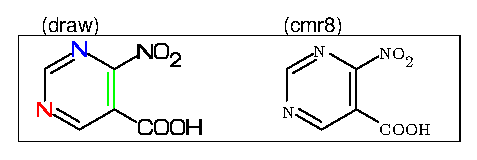
\includegraphics{mcf_man_soc-064.eps}%  for dvipdfmx
%%%%\hspace{5mm}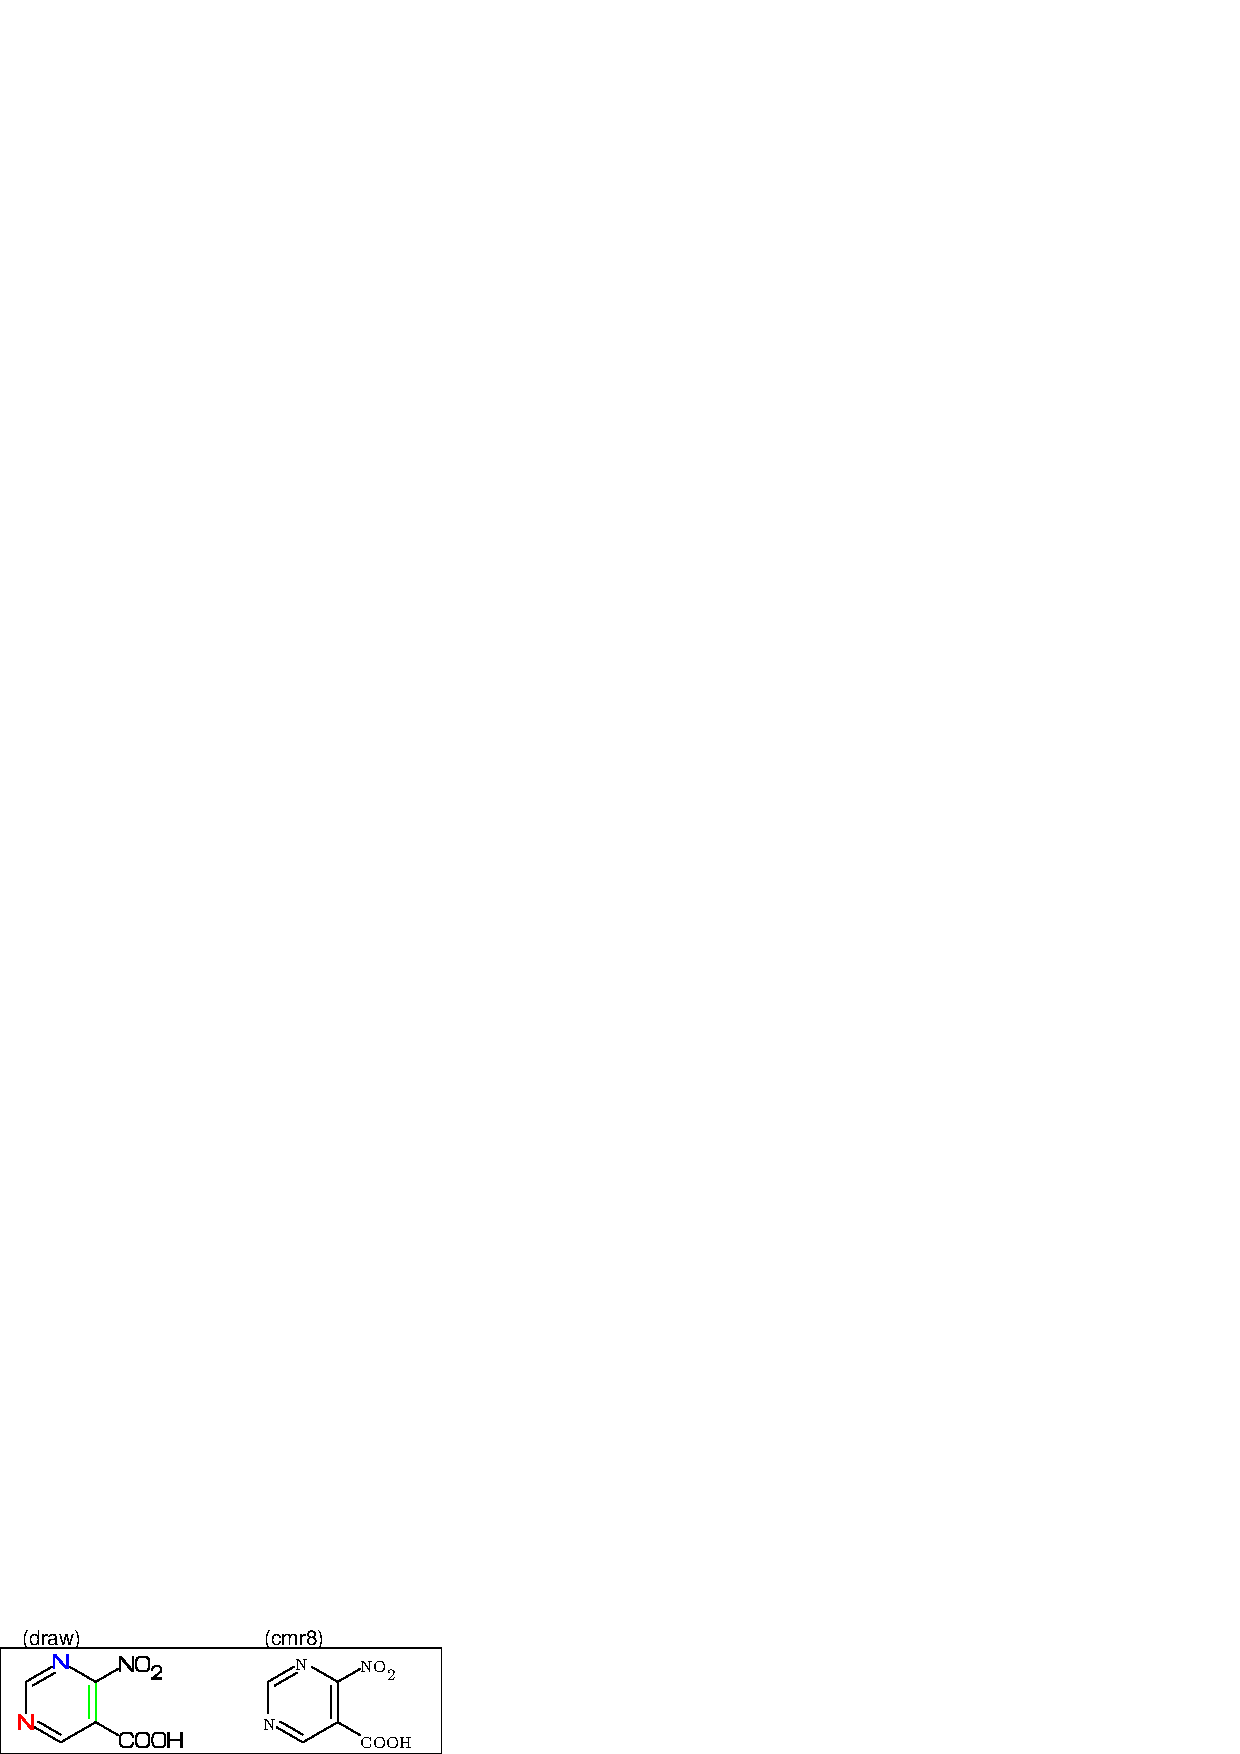
\includegraphics[width=7cm]{mcf_man_soc-064.png}%  for dvipdfmx
%%%%\MCFstructure   % for Metafont
\advance\fontnum\@ne\relax\advance\tempnum\@ne\relax%
%-----------------------------------------------------------------------------
\subsubsection{Make block}
\begin{verbatim}
  |< : start brock
  >| : end brock

  <30,!2,|<,``1.2,!2,>|,!2
\end{verbatim}
\MCFstructure
%-----------------------------------------------------------------------------
\subsubsection{Chain start multiple characters}
\begin{verbatim}
  if chain start multi charactor string,
  use !0 instead of !

  MCf(<30,COOH,!0,!3,COOH)
\end{verbatim}
\MCFstructure
\begin{verbatim}
  MCf(<30,COOH,!4,COOH)
\end{verbatim}
\MCFstructure
%-----------------------------------------------------------------------------
\subsubsection{User definition}
\begin{verbatim}
  user defined substructure
   iBuOH:='(!,/_,!,OH)
   <30,?6,{4,6}:/iBuOH
\end{verbatim}
\MCFstructure
%-----------------------------------------------------------------------------
\begin{verbatim}
  Insert user defined substructure
   <30,!3,/'(!,/_,!,OH),!3
\end{verbatim}
\MCFstructure
%%%%%%%%%%%%%%%%%%%%%%%%%%%%%%%%%%%%%%%%%%%%%%%%%%%%%%%%%%%%%%%%%%%%%%%%%%%%%%%
\newpage
\section{Option parameter}
%------------------------------------------------------------------------------
\subsection{Size parameter}
\subsubsection{Font size}
\begin{verbatim}
  beginfont("EN:Caffeine")
    font_wd:=30mm;  %<==font width
    font_ht:=20mm;  %<==font height
    MCf(<30,?6,-4=?5,{3,8}=dl,{2,6,7,9}:N,
       {2,6,9}:/_,{1,5}://O)  endfont
\end{verbatim}
\MCFstructure
%-----------------------------------------------------------------------------
\subsubsection{Margin left and right}
\begin{verbatim}
 default: margin_left_right=0.4mm
\end{verbatim}
\MCFstructure
\begin{picture}(12,20)
\put(1,14){\makebox(10,6)[r]{\tt 0mm}}
\put(1, 7){\makebox(10,6)[r]{\tt 0.4mm}}
\put(1, 0){\makebox(10,6)[r]{\tt 5mm}}
\end{picture}
%-----------------------------------------------------------------------------
\subsubsection{Margin top and bottom}
\begin{verbatim}
 default: margin_top_bottom=0.4mm
\end{verbatim}
\MCFstructure
\vspace{-3mm}%
\begin{verbatim}
      0mm       0.4mm       5mm
\end{verbatim}
%-----------------------------------------------------------------------------
\subsubsection{Offset thickness of bond}
\begin{verbatim}
  default: offset_thickness=0.2pt
\end{verbatim}
\MCFstructure
\vspace{-3mm}%
\begin{verbatim}
      0pt       0.2pt       0.5pt
\end{verbatim}
%-----------------------------------------------------------------------------
\subsubsection{Offset of doublebond gap}
\begin{verbatim}
  default: offset_bond_gap=0.3pt
\end{verbatim}
\MCFstructure
\vspace{-3mm}%
\begin{verbatim}
      0.0pt      0.3pt      1.0pt
\end{verbatim}
%-----------------------------------------------------------------------------
\subsubsection{Offset of atom width}
\begin{verbatim}
  default: offset_atom=0.8pt
\end{verbatim}
\MCFstructure
\vspace{-3mm}%
\begin{verbatim}
      0.0pt      0.8pt      2.0pt
\end{verbatim}
%-----------------------------------------------------------------------------
\subsubsection{Offset of wedge width}
\begin{verbatim}
  default:  offset_wedge=0.4pt
\end{verbatim}
\MCFstructure
\vspace{-3mm}%
\begin{verbatim}
      0.0pt      0.4pt      1.0pt
\end{verbatim}
%-----------------------------------------------------------------------------
\subsubsection{Max bond length}
\begin{verbatim}
  default:  max_bond_length=10mm
\end{verbatim}
\MCFstructure
\vspace{-3mm}%
\begin{verbatim}
     6mm       8mm         20mm
\end{verbatim}
%-----------------------------------------------------------------------------
\subsection{Ratio parameter}
%-----------------------------------------------------------------------------
\subsubsection{Thickness/bond length}
\begin{verbatim}
  default:  ratio_thickness_bond=0.015
\end{verbatim}
\MCFstructure
\vspace{-3mm}%
\begin{verbatim}
      0.005      0.015      0.030
\end{verbatim}
%-----------------------------------------------------------------------------
\subsubsection{Char/bond thickness}
\begin{verbatim}
  default:  ratio_char_bond=1.5
\end{verbatim}
\MCFstructure
\vspace{-3mm}%
\begin{verbatim}
      1.0        1.5        2.0
\end{verbatim}
%-----------------------------------------------------------------------------
\subsubsection{Bondgap/bond length}
\begin{verbatim}
  default:  ratio_bondgap_bond= 0.15
\end{verbatim}
\MCFstructure
\vspace{-3mm}%
\begin{verbatim}
      0.10       0.15       0.20
\end{verbatim}
%-----------------------------------------------------------------------------
\subsubsection{Atom/bond length}
\begin{verbatim}
  default:  ratio_atom_bond= 0.36
\end{verbatim}
\MCFstructure
\vspace{-3mm}%
\begin{verbatim}
       0.25      0.36      0.46
\end{verbatim}
%-----------------------------------------------------------------------------
\subsubsection{Wedge/bond length}
\begin{verbatim}
  default:  ratio_wedge_bond=0.12
\end{verbatim}
\MCFstructure
\vspace{-3mm}%
\begin{verbatim}
      0.10       0.12       0.20
\end{verbatim}
%-----------------------------------------------------------------------------
\subsubsection{Font atom gap/atom length}
\begin{verbatim}
  default:  ratio_atomgap_atom= 0.050
\end{verbatim}
\MCFstructure
\vspace{-3mm}%
\begin{verbatim}
      0.0       0.050       0.12
\end{verbatim}
%-----------------------------------------------------------------------------
\subsubsection{Chain/ring length}
\begin{verbatim}
  default:  ratio_chain_ring= 0.66
\end{verbatim}
\MCFstructure
\vspace{-3mm}%
\begin{verbatim}
       0.4         0.65        1.0
\end{verbatim}
%-----------------------------------------------------------------------------
\subsubsection{Zebra gap/bond length}
\begin{verbatim}
  default:  ratio_zebragap_bond=0.12
\end{verbatim}
\MCFstructure
\vspace{-3mm}%
\begin{verbatim}
       0.06      0.12      0.20
\end{verbatim}
%-----------------------------------------------------------------------------
\subsection{Drawing mode}
%-----------------------------------------------------------------------------
\subsubsection{Numbering atom}
\begin{verbatim}
  numberA_start:=3; numberA_end:=8;
  default: sw_numberA=0 :
    numberA_start=1 numberA_end=4095
\end{verbatim}
\MCFstructure
\begin{picture}(5,20)
\put(0,14){\makebox[5mm]{\tt 1}}
\put(0, 8){\makebox[5mm]{\tt 2}}
\put(0, 2){\makebox[5mm]{\tt 3}}
\end{picture}
%-----------------------------------------------------------------------------
\subsubsection{Numbering bond}
\begin{verbatim}
  numberB_start:=3; numberB_end:=8;
  default: sw_numberB=0 :
    numberB_start=1 numberB_end=4095
\end{verbatim}
\MCFstructure
\begin{picture}(5,20)
\put(0,14){\makebox[5mm]{\tt 1}}
\put(0, 8){\makebox[5mm]{\tt 2}}
\put(0, 2){\makebox[5mm]{\tt 3}}
\end{picture}
%-----------------------------------------------------------------------------
\subsubsection{Clipping mode}
\begin{verbatim}
  sw_clip:=0;
  MCd(1,0.7)(0.2,0.3)(Ph)
  MCd(1,0.7)(0.8,0.7)(Ph)
  ** default: sw_clip=0
\end{verbatim}
\MCFstructure
\begin{verbatim}
  sw_clip:=1;
  MCd(1,0.7)(0.2,0.3)(Ph)
  MCd(1,0.7)(0.8,0.7)(Ph)
\end{verbatim}
\MCFstructure
%-----------------------------------------------------------------------------
\subsubsection{Solid mode}
\begin{verbatim}
  (fit to font size)
  sw_solid=0   ** default
\end{verbatim}
\MCFstructure
%-----------------------------------------
\begin{verbatim}
  (solid ratio bond/font width)
  sw_solid:=1;
  ratio_bond_width=0.1
  font_width=60mm
  (bond_len=60mm*0.1=6mm)
  ** ignore bond_len
\end{verbatim}
\MCFstructure
%-----------------------------------------
\begin{verbatim}
  (solid bond length)
  sw_solid:=2; 
  bond_len=10mm
  ** ignore ratio_bond_width
\end{verbatim}
\MCFstructure
%-----------------------------------------
\begin{verbatim}
  (solid bond length and clip)
  sw_solid:=2;
  sw_clip:=1;
  bond_len=10mm
\end{verbatim}
\MCFstructure
%-----------------------------------------------------------------------------
\subsubsection{Expand mode}
\begin{verbatim}
  default:  sw_expand=0
\end{verbatim}
\MCFstructure\\
\makebox[5mm]{}%
\makebox[30mm]{\tt 0 :default}%
\makebox[30mm]{\tt 1}%
%-----------------------------------------------------------------------------
\subsubsection{Substituent off mode}
\begin{verbatim}
  default:  sw_subst_off=0
\end{verbatim}
\MCFstructure\\
\makebox[5mm]{}%
\makebox[30mm]{\tt 0 :default}%
\makebox[30mm]{\tt 1}%
%-----------------------------------------------------------------------------
\subsubsection{Single bond mode}
\begin{verbatim}
  default:  sw_bond_single=0
\end{verbatim}
\MCFstructure\\
\makebox[5mm]{}%
\makebox[30mm]{\tt 0 :default}%
\makebox[30mm]{\tt 1}%
%-----------------------------------------------------------------------------
\subsection{Frame}
%-----------------------------------------------------------------------------
\subsubsection{Font frame}
\begin{verbatim}
  (Draw font frame)
  margin_left_right:=5mm;
  margin_top_bottom:=2mm;
  sw_font_frame:=1;
  MCf(<30,Ph,4:/Cl,3:/F)
\end{verbatim}
\MCFstructure
\begin{verbatim}
  (Draw frame inside margin)
  sw_font_frame=2
\end{verbatim}
\MCFstructure
\begin{verbatim}
  (Draw both frame)
  sw_font_frame=3
\end{verbatim}
\MCFstructure
%-----------------------------------------------------------------------------
\subsubsection{Molecular frame}
\begin{verbatim}
  sw_mol_frame:=1;
  MCd(1,.5)(1,0.5)(<30,Ph,4:/Cl,3:/F)
  ** default: sw_mol_frame=0
\end{verbatim}
\MCFstructure
%-----------------------------------------------------------------------------
\subsubsection{Atom frame}
\begin{verbatim}
  sw_atom_frame:=1;
  MCf(<30,COOH,!0,COOH)
  ** default: sw_atom_frame=0
\end{verbatim}
\MCFstructure
%-----------------------------------------------------------------------------
\subsection{Local parameter setting}
\begin{verbatim}
  beginfont()
    MCf(Ph)
  endfont
  beginfont()
    %--------------------------
    ratio_thickness_bond:=0.05;
    %--------------------------
    MCf(Ph)
  endfont
  beginfont()
    MCf(Ph)
  endfont
\end{verbatim}
\MCFstructure\MCFstructure\MCFstructure
%-----------------------------------------------------------------------------
\subsection{Global parameter setting}
\begin{verbatim}
  beginfont()
    MCf(Ph)
  endfont
  %--------------------------
  ratio_thickness_bond:=0.05;
  %--------------------------
  beginfont()
    MCf(Ph)
  endfont
  beginfont()
    MCf(Ph)
  endfont
\end{verbatim}
\MCFstructure\MCFstructure\MCFstructure
%%%%%%%%%%%%%%%%%%%%%%%%%%%%%%%%%%%%%%%%%%%%%%%%%%%%%%%%%%%%%%%%%%%%%%%%%%%%%%%
\newpage
\section{Function}
\subsection{Function MCd()}
\begin{verbatim}
  (Draw molecule)

  MCd(a,b)(c,d)(...)
    a: ratio molecular width/font width
    b: ratio molecular hight/font hight
    c: x axis position
    d: y axis position

  beginfont()
    MCd(1,0.8)(0.2,0.9)(<30,Ph,3:/F,4:/Cl)
    MCd(1,0.8)(0.8,0.1)(<30,Ph,3:/F,4:/Cl)
  endfont
\end{verbatim}
\MCFstructure
%-----------------------------------------------------------------------------
\subsection{Function MCa()}
\begin{verbatim}
  (Draw molecule at (x,y))

  MCa(a,b)(...) : MCd(1,1)(a,b)(...)
    a: x axis position
    b: y axis position

  beginfont()
    MCa(0.2,0.5)(<30,Ph,3:/F,4:/Cl)
    MCa(0.8,0.5)(<30,Ph,3:/F,4:/Cl)
  endfont
\end{verbatim}
\MCFstructure
%-----------------------------------------------------------------------------
\subsection{Function MCc()}
\begin{verbatim}
  (Draw molecule to center of font)

  MCc(a,b)(...) : MCd(a,b)(0.5,0.5)(...)
    a: ratio molecular width/font width
    b: ratio molecular hight/font hight

  beginfont()
    MCc(1,1)(<30,?6)
    MCc(0.5,0.5)(<30,?6)
  endfont
\end{verbatim}
\MCFstructure
%-----------------------------------------------------------------------------
\subsection{Function MCf()}
\begin{verbatim}
  (Draw molecule fit to font size)

  MCf(...) : MCd(1,1)(0.5,0.5)(...)

  (Draw molecule fit to font height)

  beginfont()
    font_wd:=25mm;
    font_ht:=15mm;
    MCf(<30,Ph)
  endfont
\end{verbatim}
\MCFstructure
\begin{verbatim}

  beginfont()
    font_wd:=25mm;
    font_ht:=15mm;
    MCf(<90,Ph,3:/F,4:/Cl)
  endfont
\end{verbatim}
\MCFstructure
\begin{verbatim}

  (Draw molecule fit to font width)

  beginfont()
    font_wd:=15mm;
    font_ht:=25mm;
    MCf(<30,Ph)
  endfont
\end{verbatim}
\MCFstructure
\begin{verbatim}

  beginfont()
    font_wd:=15mm;
    font_ht:=25mm;
    MCf(<30,Ph,3:/F,4:/Cl)
  endfont
\end{verbatim}
\MCFstructure
%-----------------------------------------------------------------------------
\newpage
\subsection{Function EXT()}
\begin{verbatim}
(Add extra graphic to font)
 
 w:  font width
 h:  font height
 w0: font width-margin_left_right*2
 h0: font height-margin_top_bottom*2
 aw: atom font size
 em: label font size
 p0: x=margin_left_right
     y=margin_top_bottom
 n:  molecular number
 p[m]: molecular origin position
 w[m]: molecular width
 h[m]: molecular height

%----------------------------------------
beginfont()
 font_wd:=70mm;
 font_ht:=30mm;
 ratio_bond_width:=0.065;
 sw_solid:=1;
 %---------------------------------------
 MCd(1,1)(0.1,0.5)
  (<-210,60`1,60`1,60`1,{1,3}=dl,
   1:/R1,4:/R2^-60)
 ext(
   defaultscale:=0.6;
   label.bot("Diene",p0+(0.5w,0));
 )
 %---------------------------------------
 MCd(1,1)(0.4,0.5)
  (<-30,-60`1,1=dl,1:/R3,2:/R4^60)
 ext(
   defaultscale:=0.6;
   label.bot("Dienophile",p0+(0.5w,0));
 )
 %---------------------------------------
 MCd(1,1)(0.9,0.5)
  (<30,?6,6=dl,2:/R2,3:/R4,4:/R3,5:/R1)
 %---------------------------------------
 EXT(
   drawarrow (0.52w,0.5h)..(0.6w,0.5h);
   defaultscale:=0.7;
   label("+",(0.25w,0.5h));
   label.bot("Diels-Alder Reaction",
            (0.5w,h));
 )
 %---------------------------------------
endfont
\end{verbatim}
\MCFstructure
%-----------------------------------------------------------------------------
\newpage
\subsection{Function ext()}
\begin{verbatim}
(Add extra graphic to molecule)

 w:       molecular width
 h:       molecular height
 aw: atom font size
 em: label font size
 p0:      origin of molecular structure
 l:       bond length
 An:      atom number
 A[m]:    atom position
 A[m]dir: branch direction of A[m]
 Bn:      bond number
 B[m]s:   bond start position
 B[m]e:   bond end position
 B[m]:    bond position(0.5[B[m]s,B[m]e])
 B[m]dir: bond direction

%----------------------------------------
beginfont()
  font_wd:=50mm;
  font_ht:=20mm;
 %---------------------------------------
  MCd(1,0.7)(0,0.5)(<30,?6,3=dl,4:/CH3)
  ext(
    label.top("+",A7);
    drawarrow B3{dir(B3dir-90)}..
              {dir(B7dir+90)}0.4[B7s,B7e];
    )
 %---------------------------------------
  MCd(1,0.7)(1,0.5)(<30,?6,4://CH3)
  ext(
    labeloffset:=0bp;
    label.lrt("+",A3);
  )
 %---------------------------------------
  EXT(
    drawdblarrow (0.4w,0.5h)..(0.55w,0.5h);
  )
 %---------------------------------------
endfont
\end{verbatim}
\MCFstructure
\begin{verbatim}
label:
 defaultfont: label font
 defaultfont="draw": draw font
 **default defaultfont="draw"

drawarrow & drawdblarrow:
 sw_arrow=0: emulation mode
 sw_arrow=1: plain.mp mode
 **default sw_arrow=0
\end{verbatim}
%-----------------------------------------------------------------------------
\newpage
\section{MCF example}
%-----------------------------------------------------------------------------
\subsection{Acetamiprid}
\begin{verbatim}
  <30,Ph,2:N,1:/Cl,
     4:\,!,N,/_,!,/_,!!,N,!,CN
\end{verbatim}
\MCFstructure
%-----------------------------------------------------------------------------
\subsection{Fenitrothion}
\begin{verbatim}
  <30,!,O,!,P,//S,/O!^160,!,O,!,
      |,Ph,3:/_,4:/NO2
\end{verbatim}
\MCFstructure
%-----------------------------------------------------------------------------
\subsection{Permethrin}
\begin{verbatim}
  <-30,?3,2^-35:*/_,2^35:/*_,
     1:\,!!,/Cl,!,Cl,
     3:\,//O,!,O,!2,Ph,
    -4:\,O,-60,Ph
\end{verbatim}
\MCFstructure
%-----------------------------------------------------------------------------
\subsection{Endosulfan}
\begin{verbatim}
  <26,?7,7=?6[13],11:@,208~wf`1.45,8~wb:&,
      10=d,{3,5}:O,4:S,4://O,
      {8,9,10,11,12^-210,12^-150}:/Cl
\end{verbatim}
\MCFstructure
%-----------------------------------------------------------------------------
\subsection{Luciferin}
\begin{verbatim}
  <30,Ph,3=?5,8:\,?5,{9,16}=dl,
     {9,14}:N,{7,11}:S,
     1:/OH,-2:*/COOH
\end{verbatim}
\MCFstructure
%-----------------------------------------------------------------------------
\subsection{Warfarin}
\begin{verbatim}
  <30,Ph,3=?6,8=dl,
  10:O,7:/OH,9://O,
  8:\,/Ph`1,60,!,//O,!
\end{verbatim}
\MCFstructure
%-----------------------------------------------------------------------------
\subsection{Limonin}
\begin{verbatim}
 <30,?6,{-3,-4}=?6,-5=?3,
  -2=wf,-1=wb,6=?5,-4=?6,-5=wf,
  {13,15,17,20}:O,{3,12,21}://O,
  {4~wf^60,8~zf^60,18^35,18^-35}:/_,
  {1^60,5^180,16^60}:/*H,
  14:\*,|,?5,{1,4}=dl,3:O
\end{verbatim}
\MCFstructure
%-----------------------------------------------------------------------------
\subsection{Sesamine}
\begin{verbatim}
 <54,?5,1=?5,
 {4,7}:O,{1^-54,2^54}:*/H,
 5:*\^-12,Ph,-3=?5,{-1,-3}:O,
 8:*\^-12,Ph,-3=?5,{-1,-3}:O
\end{verbatim}
\MCFstructure
%-----------------------------------------------------------------------------
\subsection{Colchicine}
\begin{verbatim}
  <30,Ph,{1,2,6}:/O!,
  -4=?7,-5=?7,
  {-1,-4,-6}=dl,-2://O,-3:/O!,
  9:\,NH,!,//O,!
\end{verbatim}
\MCFstructure
%-----------------------------------------------------------------------------
\subsection{Lycorine}
\begin{verbatim}
  <30,Ph,
  -4=?6,-2=?6,6=?5,(9,12)=?5[3],
  13=dl,
  8:N,{15,17}:O,
  9:/*H^180,10:*/H^60,
  13:*/OH,14:/*OMe
\end{verbatim}
\MCFstructure
%-----------------------------------------------------------------------------
\subsection{Gibberellin}
\begin{verbatim}
  <18,?5,3=?7,5=?6[12],
  8:@,160`1.3,3:&,
  13=dl,6=wf,8=wb,
  5:@,40~zf`1,O,60,//O^180,14~zb:&,
  2:/COOH,7://_,13:*/OH,8:/*OH,
  14:*/_,{1^60,4^60}:*/H
\end{verbatim}
\MCFstructure
%-----------------------------------------------------------------------------
\subsection{Quinine}
\begin{verbatim}
  <30,Ph,3=Ph,7:N,6:/O!,
   10:\,*/OH,/H~zf^-60,!,
   |,?6,2:N,1:*/H^60,
   4:*\,!!,
   2:@,165~zf,60,5~zb:&
\end{verbatim}
\MCFstructure
%-----------------------------------------------------------------------------
\subsection{Atoropin}
\begin{verbatim}
  <-30,O,!,//O,!,!,Ph,
  $1:@,-120~zb,
  |,?7,6:*\^190`1.02,N,/_,3~wb:&,
  $3:\~wv,!,OH
\end{verbatim}
\MCFstructure
%-----------------------------------------------------------------------------
\subsection{Rotenone}
\begin{verbatim}
  <-60,?5,{-3,-2,-3,-4}=?6,
  {7,9,-2,-4}=dl,{3,17}=dr,
  {2,13,16}:O,10://O,{11^-60,12^60}:*/H,
  {-2,-3}:/O!,1:*\,/_,!!
\end{verbatim}
\MCFstructure
%-----------------------------------------------------------------------------
\subsection{Pyrethrin I}
\begin{verbatim}
  <30,?3,{3^35~wf,3^-35~zf}:/_,
  1:*\,!!,iPr,2:\*,//O,!,O,-36~zb,|,
  ?5,-2=d,-1:/_,-3://O,-2\,!4,{-1,-3}=dl
\end{verbatim}
\MCFstructure
%-----------------------------------------------------------------------------
\subsection{Validamycin}
\begin{verbatim}
  <30,?6,{5,6}:/OH,3:/!OH>rl,
  $4:\,O,-60,|,?6,2:O,{3,4,5}:/OH,6:/!OH,
  $1:\,NH,!,|,?6,2=dl,{4,5,6}:/OH,3:/!OH
\end{verbatim}
\MCFstructure
%-----------------------------------------------------------------------------
\subsection{Paclitaxel}
\begin{verbatim}
  ?6,5=d,3:@,|<,``1,36,45,45,45,45,>|,$5:&,
  -4=?6,-4=?4,-1=wb,-3=wf,-1:O,||,
  {4^35,4^-35,6}:/_,{3^-60,15}:*/OH,
  8:/*H^-60,9:*/_^60,10://O,
  1:\,O,!,//O,!,*/OH,!,/Ph,
  60~wf,NH,-60,//O,60,Ph,
  7:\*,O,-45,//O,60,Ph,11:*\,O,-60,//O,60,
 12:\*^-15,O,60,//O,-60
\end{verbatim}
\MCFstructure
%-----------------------------------------------------------------------------
\onecolumn
\section{Example to use mcf2graph}
\subsection{Molecular definition file}
\begin{verbatim}
%-------------------------------------------------------------------------
input mcf2graph.mf;                               % input macro
%-------------------------------------------------------------------------
sw_auxout:=1;         % aux(information) file output on > Gloval setting
font_wd:=60mm;        % font width                      > 
font_ht:=40mm;        % font height                     >
var3:="cal_MW"; tag3:="cMW";                            > AUX file table
var4:="cal_FM"; tag4:="cFM";                            >
%%%% sw_report:=1;                                      > Report output
%%%% sw_MOLout:=1;                                      > MOL file output
outputformat:="png"; hppp:=vppp:=0.1;                   > PNG output
outputtemplate:="%j-%3c.png";                           >
%-------------------------------------------------------------------------
beginfont("NO:1","EN:Ampicillin")                 > begin font(information)
  MCf(<45,?4,2:N,2=?5,-1:S,                             > begin MCF (1)
     {3^45,4^-45}:/*H,1://O^15,5:/*COOH^-18,            >
     {6^35,6^-35}:/_,                                   >
     4:@,75,NH,!,//O,!,/*NH,!,Ph)                       > end MCF 
endfont                                                 > end font
%------------------------------------------------------------------------
beginfont("NO:2","EN:Cholesterol")                > begin font(information)
  MCf(<30,?6,{-4,-2}=?6,-4=?5,7=dl,                     > begin MCF (2)
      1:*/OH,{4,12}:*/_^60,9:*/H^60,                    >
      10:/*H^180,{11,-1}:/*H^-60,                       >
      -1:@,17,/*_,!4,/_,!)                              > end MCF
endfont                                                 > end font
%------------------------------------------------------------------------
beginfont("NO:3","EN:Limonin")                    > begin font(information)
  MCf(<30,?6,{-3,-4}=?6,                                > begin MCF (3)
      -5=?3,-2=wf,-1=wb,6=?5,-4=?6,-5=wf,               >
      {13,15,17,20}:O,{3,12,21}://O,                    >
      {4~wf^60,8~zf^60,18^35,18^-35}:/_,                >
      {1^60,5^180,16^60}:/*H,                           >
      14:\*,|,?5,{1,4}=dl,3:O)                          > end MCF
endfont                                                 > end font
%------------------------------------------------------------------------
beginfont("NO:4","EN:beta-carotene)               > begin font(information)
  MCf(<30,?6,3=dl,{3,5^35,5^-35}:/_,                    > begin MCF (4)
      4:\,|,!18,{1,3,5,7,9,11,13,15,17}=dr,             >
      {3,7,12,16}:/_,                                   >
      |,?6,6=dl,{6,2^35,2^-35}:/_)                      > end MCF
endfont                                                 > end font
%------------------------------------------------------------------------
beginfont("NO:5","EN:Gibberellin A3");            > begin font(information)
  MCf(<18,?5,3=?7,5=?6[12],                             > begin MCF (5)
     8:@,160`1.3,3:&,13=dl,6=wf,8=wb,                    >
     5:@,40~zf`1,O,60,//O^180,14~zb:&,                   >
     2:/COOH,7://_,13:*/OH,8:/*OH,                      >
     14:*/_,{1^60,4^60}:*/H)                            > end MCF
endfont;                                                > end font
%------------------------------------------------------------------------
bye
\end{verbatim}
%------------------------------------------------------------------------
\noindent%
\newpage
\subsection{Information auxfile output}
\paragraph{(Insert option parameter setting)}
\begin{verbatim}
  sw_auxout:=1;
  ** default : sw_auxout=0
\end{verbatim}
\paragraph{(Command line)}
\begin{verbatim}
  >mpost -s ahangle=0 FILENAME (molecular definition file)
\end{verbatim}
\paragraph{(Sourse)}
\begin{verbatim}
beginfont("EN:Ampicillin")(....)
beginfont("EN:Cholesterol")(....)
beginfont("EN:Limonin")(....)
beginfont("EN:beta-Carotene")(....)
beginfont("EN:Gibberellin A3")(....)
\end{verbatim}
\paragraph{(Setting)}
\begin{verbatim}
tag1:="F";   var1:="jobname";     * default output
tag2:="C";   var2:="char_num";    * default output
tag3:="cMW"; var3:="calc_weight";
tag4:="cFM"; var4:="calc_formula";
\end{verbatim}
\paragraph{(Output)}
\begin{verbatim}
(sw_auxfix=0)
F:mcf_man_soc;C:1;cMW:349.40462;cFM:C16H19N3O4S;EN:Ampicillin
F:mcf_man_soc;C:2;cMW:386.6532;cFM:C27H46O;EN:Cholesterol
F:mcf_exa_soc;C:3;cMW:470.5113;cFM:C26H30O8;EN:Limonin
F:mcf_exa_soc;C:4;cMW:536.8722;cFM:C40H56;EN:beta-Carotene
F:mcf_exa_soc;C:5;cMW:346.3742;cFM:C19H22O6;EN:Gibberellin A3

(sw_auxfix=1)
F;C;cMW;cFM;EN
mcf_man_soc;1;349.40462;C16H19N3O4S;Ampicillin
mcf_man_soc;2;386.6532;C27H46O;Cholesterol
mcf_exa_soc;3;470.5113;C26H30O8;Limonin
mcf_exa_soc;4;536.8722;C40H56;beta-Carotene
mcf_exa_soc;5;346.3742;C19H22O6;Gibberellin A3

(aux_delimiter:="/";)
F:mcf_man_soc/C:1/cMW:349.40462/cFM:C16H19N3O4S/EN:Ampicillin
F:mcf_man_soc/C:2/cMW:386.6532/cFM:C27H46O/EN:Cholesterol
F:mcf_exa_soc/C:3/cMW:470.5113/cFM:C26H30O8/EN:Limonin
F:mcf_exa_soc/C:4/cMW:536.8722/cFM:C40H56/EN:beta-Carotene
F:mcf_exa_soc/C:5/cMW:346.3742/cFM:C19H22O6/EN:Gibberellin A3
\end{verbatim}
\paragraph{(Tag)}
\begin{verbatim}
F   : filename
C   : char number
NO  : serial number
EN  : english name
JN  : japanese name
FM  : formula from literature data
MW  : molecular weight from literature data
USE : the use
cMW : molecular weight calculated
cMI : monoisotopic mass calculated
cFM : molecular formula calculated
\end{verbatim}
%------------------------------------------------------------------------
\newpage
\noindent%
\subsection{Report output}
\paragraph{(Insert option parameter setting)}
\begin{verbatim}
  sw_report:=1;
  ** default : sw_report=0
\end{verbatim}
\paragraph{(Command line)}
\begin{verbatim}
  >mpost -s ahangle=0 -s ahlength=2 FILENAME (molecular definition file)
\end{verbatim}
\paragraph{(Output)}
\begin{verbatim}
------------------------------------------------------------------
 Molecular name = Nicotine
 Warnings =   0 / Expanded command = 40
 Width * Height =   49.57332 *   41.37605
 Shift width * height  =          0 *   -9.07253
 Bond length = 12.75589   Atom size   = 5.38914
 Atom count= 12 Bond count= 13 Ring count=  2 Hide H count= 14
------------------------------------------------------------------
< NO. >(  x axis   ,   y axis   )< atom  >< bond >< hide_H >
 A1    (         0 ,          0 )  C           3       1
 A2    (     0.866 ,       -0.5 )  N           3
 A3    (     1.732 ,          0 )  C           3       1
 A4    (     1.732 ,          1 )  C           4
 A5    (     0.866 ,        1.5 )  C           3       1
 A6    (         0 ,          1 )  C           3       1
 A7    (     2.304 ,       1.33 )  C           3       1
 A8    (     3.217 ,      0.923 )  N           3
 A9    (     3.886 ,      1.666 )  C           2       2
 A10   (     3.386 ,      2.532 )  C           2       2
 A11   (     2.408 ,      2.325 )  C           2       2
 A12   (     3.399 ,      0.067 )  C           1       3
------------------------------------------------------------------
< NO. ><  bond   (sdt)><angle + (  +-  )><length (   pt   )>
 B1     1 ->   2 (  2)      330 (   -30)       1 (   12.76)
 B2     2 ->   3 (  1)       30 (    30)       1 (   12.76)
 B3     3 ->   4 (  2)       90 (    90)       1 (   12.76)
 B4     4 ->   5 (  1)      150 (   150)       1 (   12.76)
 B5     5 ->   6 (  2)      210 (  -150)       1 (   12.76)
 B6     6 ->   1 (  1)      270 (   -90)       1 (   12.76)
 B7     4 ->   7 (  1)       30 (    30)    0.66 (    8.42)
 B8     7 ->   8 (  1)      336 (   -24)       1 (   12.76)
 B9     8 ->   9 (  1)       48 (    48)       1 (   12.76)
 B10    9 ->  10 (  1)      120 (   120)       1 (   12.76)
 B11   10 ->  11 (  1)      192 (  -168)       1 (   12.76)
 B12   11 ->   7 (  1)      264 (   -96)       1 (   12.76)
 B13    8 ->  12 (  1)      282 (   -78)    0.66 (    8.42)
------------------------------------------------------------------
<atom>( atom wt )[ mi wt   ]  < cnt > < sum wt   >[ sum mi wt  ]
 C    (  12.0107)[       12] *   10 =    120.10696[         120]
 H    (  1.00793)[  1.00783] *   14 =     14.11108[    14.10959]
 N    (  14.0067)[ 14.00307] *    2 =      28.0134[    28.00613]
 Molecular Weight  [Mono Isotopic]  =     162.2314[   162.11572]
------------------------------------------------------------------
 Weight  Calc: 162.2314 / Input: 162.23 / weight gap= 0.00145
 Fomula  Calc: C10H14N2 / Input: 
==================================================================
\end{verbatim}%
\newpage
%------------------------------------------------------------------------
\noindent%
\subsection{Molfile output}
\paragraph{(Insert option parameter setting)}
\begin{verbatim}
  sw_MOLout:=1;
  ** default : sw_MOLout=0
\end{verbatim}
\paragraph{(Command line)}
\begin{verbatim}
  >mpost -s ahangle=3  FILENAME (molecular definition file)
\end{verbatim}
\paragraph{(Output)}
\begin{verbatim}
%%%%%%%%%%%%%%%%%%%%%%%%%%%%%%%%%%%%%%%%%%%%%%%%%%%%%%%%%%%%%%%%%%%%%
  -MCFtoMOL- EN:Caffeine         

 14 15  0  0  0  0  0  0  0  0999 V2000
         0         0         0 C   0  0  0  0
   0.86603      -0.5         0 N   0  0  0  0
   1.73206         0         0 C   0  0  0  0
   1.73206         1         0 C   0  0  0  0
   0.86603       1.5         0 C   0  0  0  0
         0         1         0 N   0  0  0  0
    2.6831  -0.30902         0 N   0  0  0  0
   3.27089       0.5         0 C   0  0  0  0
    2.6831   1.30902         0 N   0  0  0  0
   0.86603  -1.36383         0 C   0  0  0  0
  -0.76894   1.44394         0 C   0  0  0  0
  -0.76894  -0.44394         0 O   0  0  0  0
   0.86603   2.36383         0 O   0  0  0  0
   2.95299    2.1396         0 C   0  0  0  0
  1  2  1  0     0  0
  2  3  1  0     0  0
  3  4  2  0     0  0
  4  5  1  0     0  0
  5  6  1  0     0  0
  6  1  1  0     0  0
  3  7  1  0     0  0
  7  8  2  0     0  0
  8  9  1  0     0  0
  9  4  1  0     0  0
  2 10  1  0     0  0
  6 11  1  0     0  0
  1 12  2  0     0  0
  5 13  2  0     0  0
  9 14  1  0     0  0
M  END
%%%%%%%%%%%%%%%%%%%%%%%%%%%%%%%%%%%%%%%%%%%%%%%%%%%%%%%%%%%%%%%%%%%%%
\end{verbatim}%
%----------------------------------------------------------------------------
\newpage
\subsection{LuaTeX file example}
%############################################################################
\begin{verbatim}
%--------------------------------------------------------------------
\documentclass{article}
\usepackage{luamplib}%
\mplibcodeinherit{enable}%
\mplibverbatim{enable}%
\everymplib{if unknown Ph1:
              input mcf2graph.mf;
              mp_log_name:="temp-info.aux";
              sw_auxout:=1; 
            fi}%
%--------------------------------------------------------------------
\begin{document}
\noindent%
%--------------------------------------------------------------------
\begin{mplibcode}
  font_wd:=50mm; font_ht:=50mm;
  beginfont("NO:2","EN:Limonin","MW:470.51")
  MCf(<30,
    ?6,{-3,-4}=?6,
      -5=?3,-2=wf,-1=wb,6=?5,-4=?6,-5=wf,
      {13,15,17,20}:O,{3,12,21}://O,
      {4~wf^60,8~zf^60,18^35,18^-35}:/_,
      {1^60,5^180,16^60}:/*H,
      14:\*,|,?5,{1,4}=dl,3:O
  )
  endfont
\end{mplibcode}\\
%--------------------------------------------------------------------
\begin{mplibcode}
  font_wd:=80mm; font_ht:=50mm;
  beginfont("NO:3","EN:beta-carotene","MW:536.87")
    MCf(<30,
      ?6,3=dl,{3,5^35,5^-35}:/_,
      4:\,|,!18,{1,3,5,7,9,11,13,15,17}=dr,
      {3,7,12,16}:/_,
      |,?6,6=dl,{6,2^35,2^-35}:/_
    )
  endfont
\end{mplibcode}\\
%--------------------------------------------------------------------
\begin{mplibcode}
  font_wd:=50mm; font_ht:=50mm;
  beginfont("NO:4","EN:Gibberellin A3","MW:346.37");
  MCf(<18,?5,3=?7,5=?6[12],
     8:@,160`1.3,3:&,13=dl,6=wf,8=wb,
     5:@,40~zf`1,O,60,//O^180,14~zb:&,
     2:/COOH,7://_,13:*/OH,8:/*OH,
     14:*/_,{1^60,4^60}:*/H
  )
endfont;
\end{mplibcode}\\
%--------------------------------------------------------------------
\end{document}
%--------------------------------------------------------------------
\end{verbatim}%
%############################################################################
%------------------------------------------------------------------------
\newpage
\subsection{LaTeX file example}
%############################################################################
\begin{verbatim}
%--------------------------------------------------------------------
\documentclass[a4paper]{article}
\usepackage{graphicx}
\pagestyle{empty}
\makeatletter%
%--------------------------------------------------------------------
\def\@F{F}\def\@C{C}\def\@EN{EN}\def\@NO{NO}\def\@MW{MW}\def\@FMc{FMc}%
\def\@fst@param#1:#2;{#1}\def\@sec@param#1:#2;{#2}%
\def\mol@sel#1{%
\if#1\empty\relax\else%
  \edef\@tag{\expandafter\@fst@param#1;}%
  \edef\@var{\expandafter\@sec@param#1;}%
  \ifx\@tag\@F\edef\MOLfile{\@var}\fi%
  \ifx\@tag\@C\edef\MOLchar{\@var}\fi%
  \ifx\@tag\@EN\edef\MOLnameE{\@var}\fi%
  \ifx\@tag\@NO\edef\MOLnum{\@var}\fi
  \ifx\@tag\@MW\edef\CALmw{\@var}\fi
  \ifx\@tag\@FMc\edef\CALfm{\@var}\fi
\fi}%
\def\put@char{%
  \begin{picture}(84,42)%
     \put(0,38){\bf [\MOLnum]\MOLnameE{ }\small\tt/FM:\CALfm/MW:\CALmw}%
     \put(10,0){\font\@strufont=\MOLfile\relax%
               \hbox{\@strufont\char\MOLchar}}%
  \end{picture}%
\def\INFO#1{\@for\@temp:=#1\do{\mol@sel\@temp}\put@char}%
\makeatother
%--------------------------------------------------------------------
\begin{document}
\unitlength=1mm%
\INFO{F:mcf_man_soc,C:134,NO:1,cMW:349.40462,cFM:C16H19N3O4S,EN:Ampicillin}%
\INFO{F:mcf_man_soc,C:135,NO:2,cMW:386.6532,cFM:C27H46O,EN:Cholesterol}%
\end{document}
%--------------------------------------------------------------------
\end{verbatim}%
%############################################################################
%------------------------------------------------------------------------
\INFO{F:mcf_man_soc,C:134,NO:1,cMW:349.40462,cFM:C16H19N3O4S,EN:Ampicillin}%
\INFO{F:mcf_man_soc,C:135,NO:2,cMW:386.6532,cFM:C27H46O,EN:Cholesterol}%
%------------------------------------------------------------------------
\end{document}
